\section{Discussion and Comparison (Jonas, Julius)}

To discuss the effect and impact of adaptive and generative music on the player, two studies are first presented. The studies evaluate the subjective responses of the participants and compare these responses for environments with linear, adaptive or generative music.

\subsection{Study 1}
Hutchings and McCormack have adapted an AMS (adaptive music system) to the two video games "Zelda: Mystery of solarus" \cite{zeldamysteryofsolarus2011}  and "Starcraft ii: Wings of liberty" \cite{starcraftiiwingsofliberty} \cite{hutMcCormAms}. The system was integrated into the games so that it receives information about the current state of the game at runtime \cite{hutMcCormAms}. In addition, the musical output of the system was replaced with the output of the AMS \cite{hutMcCormAms}. 
The system was then evaluated in a study with 34 participants \cite{hutMcCormAms}. The participants were asked to provide information on their feeling of immersion, the quality of the music and the correlation between music and actions \cite{hutMcCormAms}. They were divided into two groups \cite{hutMcCormAms}. Group A plays the game "Zelda: Mystery of solarus" with original music and "Starcraft ii: Wings of liberty" with music from the AMS \cite{hutMcCormAms}. Group B runs through both games in the other environment \cite{hutMcCormAms}. This prevents a participant from playing one game in two different music environments and therefore reduces bias \cite{hutMcCormAms}.
Furthermore, during the evaluation, the participants were played a short section of music that represents a certain game state or is played at a certain point in the game \cite{hutMcCormAms}. The participants then had to assign a term for a concept from the game to this section of music that they thought best suit \cite{hutMcCormAms}. The four game concepts for the music sections are shown in Fig. \Cref{fig:tutorial_gal_def}. Additional the accepted terms for every concept are listed. 
\begin{figure}
    \centering
    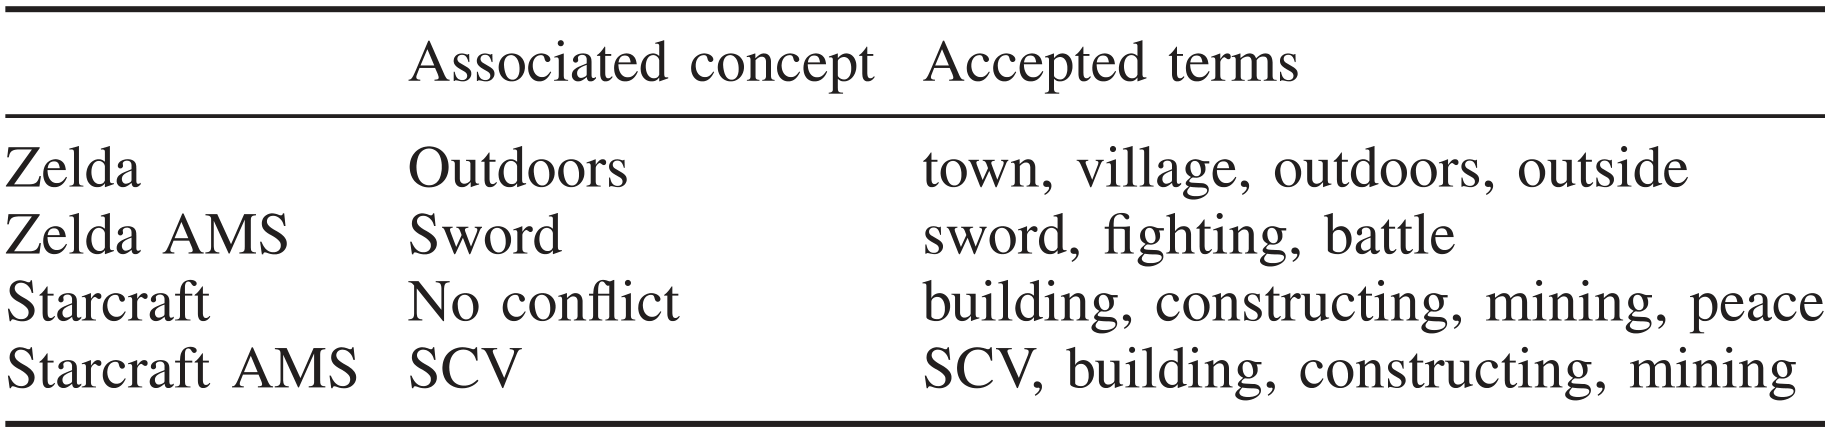
\includegraphics[width=1\linewidth]{images/ams_evaluation_table2.png}
    \caption{Accepted terms for established concepts \cite{hutMcCormAms}}
    \label{fig:ams_evaluation_table2}
\end{figure}
Participants of group A was played the music sections of the AMS conditions “Zelda AMS” and “Starcraft AMS” (see Fig \Cref{fig:tutorial_gal_def}) \cite{hutMcCormAms}. Group B was played the original music conditions “Zelda” and “Starcraft”) (see Fig. \Cref{fig:tutorial_gal_def}) \cite{hutMcCormAms}.
For the “Zelda” condition, 70\% of participants stated a correct term. For the “Zelda AMS” condition, only 53\% of the participants reported one of the terms defined as correct \cite{hutMcCormAms}.
For music from the game “Starcraft ii: Wings of liberty” the results were similar with 59\% of participants assigning a correct term to the original music and 41\% of participants assigning a correct term to the music section of the AMS \cite{hutMcCormAms}.
This indicates that music from the AMS is more often misinterpreted and the associated game context is more likely to be confused than with the original, composed music.
However, the other reported results of the participants show a significant increase in the immersion and correlation of music with the music output of the AMS compared to the original music \cite{hutMcCormAms}.
Hutchings and McCormack conclude that the AMS could be successfully applied to the games in this study \cite{hutMcCormAms}. Furthermore, they see the spreading activation model used for the AMS as a suitable model for analysing player emotions and game events \cite{hutMcCormAms}.

\subsection{Study 2}
Another study on the effects of adaptive music on the player was conducted by Plut and Pasquier \cite{plut2019music}. They created a video game called "Galactic Escape" using "FMOD Studio" \cite{fmod} to adapt the music to the gameplay \cite{plut2019music}. 25 participants took part in this study \cite{plut2019music}. Each participant played the game “Galactic defense” once with each of the four different music conditions (see Fig. \Cref{fig:music_matters_table3}). The order of the music conditions was decided at random \cite{plut2019music}.
\begin{figure}
    \centering
    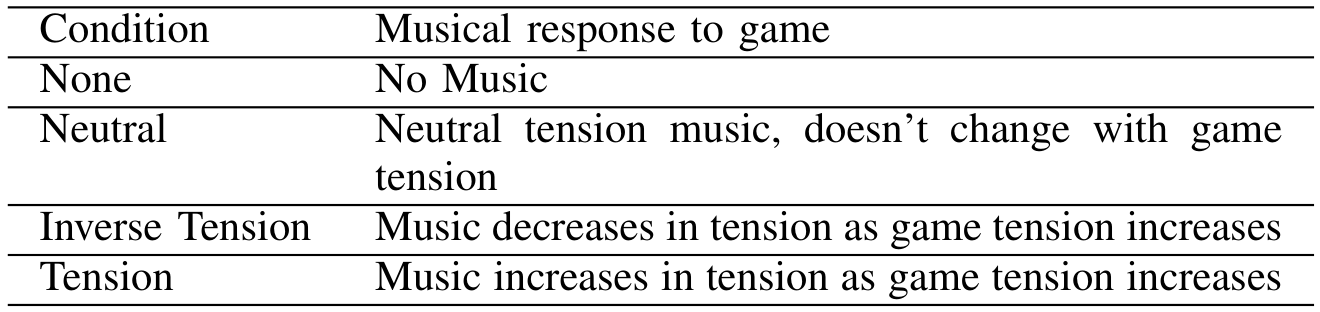
\includegraphics[width=1\linewidth]{images/music_matters_table3.png}
    \caption{Experimental conditions \cite{plut2019music}}
    \label{fig:music_matters_table3}
\end{figure}
After each game run, the participants report their enjoyment, affect and emotion by filling out a questionnaire \cite{plut2019music}. 
According to the results of the questions about enjoyment, the participants enjoyed the condition “None” (see Fig. \Cref{fig:music_matters_table3}) without music the least \cite{plut2019music}. For the other three conditions the participants reported similar response values \cite{plut2019music}.
A greater difference between the conditions was reported for the question about emotion \cite{plut2019music}. The participants indicate a higher response value for emotion in the "neutral" and "inverse tension" condition (see Fig. \Cref{fig:music_matters_table3}) compared to the condition without music \cite{plut2019music}. For the "tension" condition, which features a congruent adaptation of music to the level of tension, the emotional response value is even higher than for the other conditions \cite{plut2019music}.
For the evaluation of the player's affect, Plut and Pasquier used a three-dimensional affect model with the dimensions valence, tension and arousal, which is a simplified version based on a more complex model by Schimmack and Grob \cite{schimmack2000dimensional} \cite{plut2019music}.
The questions about the player's affect are divided in one question for each dimension \cite{plut2019music}.
The response value for the dimensions arousal and valence show a similar trend and are similar to the emotional response (see Fig. \Cref{fig:music_matters_experienced_affect}) \cite{plut2019music}. The arousal and valence value is higher for the "neutral" and "inverse tension" condition compared to the "none" condition without music \cite{plut2019music}. The values increase even further for the "tension" condition \cite{plut2019music}.
In contrast to this, the self-reported tension is decreased when music is introduced in the "neutral" condition compared to the "none" condition without music. However, it increases in the "inverse tension" and "tension" conditions, which feature adaptive music \cite{plut2019music}.
\begin{figure}
    \centering
    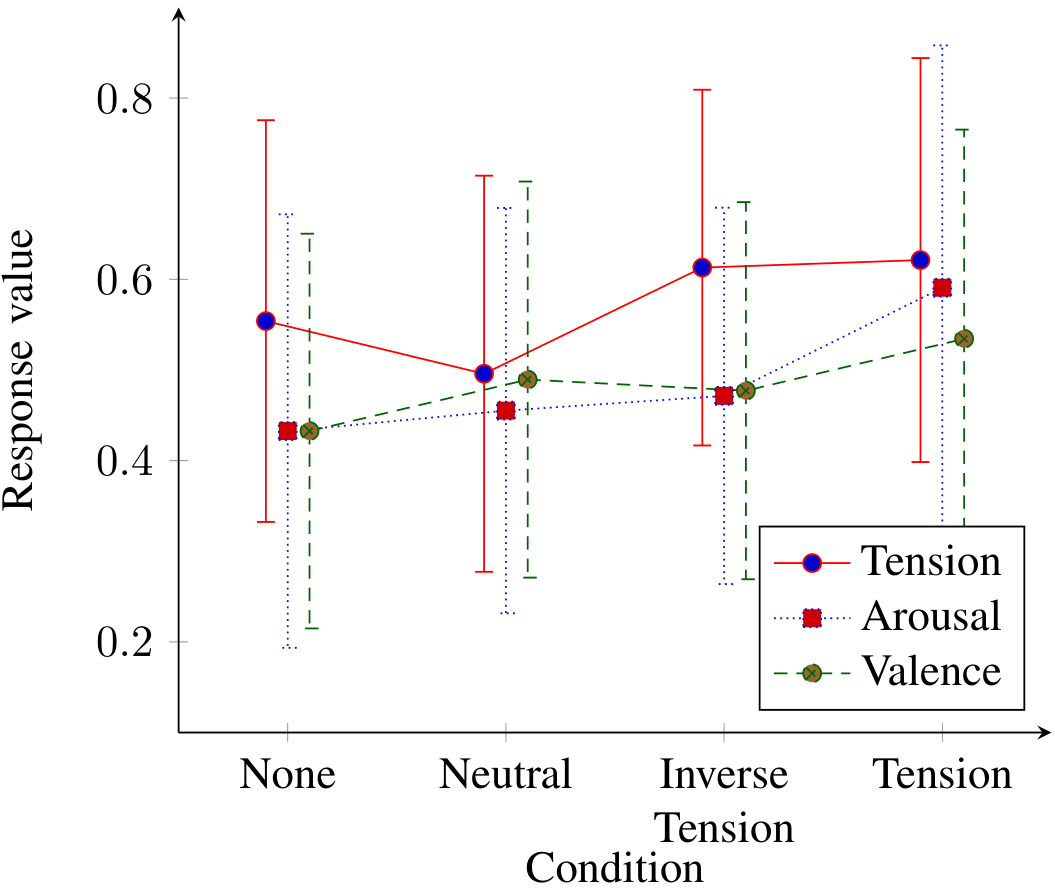
\includegraphics[width=1\linewidth]{images/music_matters_experienced_affect.png}
    \caption{Experienced affect means and Standard Deviations \cite{plut2019music}}
    \label{fig:music_matters_experienced_affect}
\end{figure}

\subsection{Study 3}
TODO: Studie aus Preglam Paper noch mit einbeziehen

Wie viel bringt welche Technik / welcher Ansatz, welches System
hat bessere Auswirkungen?

\begin{itemize}
    \item Ansichten, Meinungen/konkurrierende Ansätze vergleichen, kritisch würdigen
    \item unterschiedliche Argumentationen vorstellen/gegenüberstellen
    \item Bedeutung/Impact der wissenschaftlichen Arbeiten beschreiben, daraus folgenden Anwendungsfälle darstellen/diskutieren
    \item Nachteile, technische Begrenzungen

\end{itemize}